\documentclass[10pt,a4paper]{article}
\usepackage[spanish,es-noshorthands]{babel}
\usepackage[utf8]{inputenc}
\usepackage[T1]{fontenc}
\usepackage{lmodern}
\usepackage[a4paper,margin=2cm]{geometry}
\usepackage{amsmath,amssymb}
\usepackage{booktabs,tabularx}
\usepackage{graphicx}
\usepackage{xcolor}
\usepackage{enumitem}
\usepackage[hidelinks]{hyperref}
\usepackage{titlesec}
\titleformat{\section}{\large\bfseries\color[HTML]{1F3A60}}{\thesection.}{0.5em}{}
\titlespacing*{\section}{0pt}{8pt}{3pt}
\setlist{itemsep=1pt,topsep=2pt}
\setlength{\parskip}{3pt}
\setlength{\parindent}{0pt}
\graphicspath{{../../results/figures/}}
\newcommand{\R}{\mathcal{R}}\newcommand{\D}{\mathcal{D}}\newcommand{\G}{\mathcal{G}}
\newcommand{\F}{\mathcal{F}}\newcommand{\Lab}{\mathcal{L}}\newcommand{\Pet}{\mathcal{P}}

\begin{document}

{\LARGE\bfseries Cuadrantes de guardias médicas justos y factibles}\\[2pt]
{\large Checkpoint del modelo · Optimización y Simulación}\\[2pt]
{\small Miguel Troyano Martín · Claudia María López Bombín · María Teresa Sangil Terrés \hfill 16 de noviembre de 2026}\\[-4pt]
\rule{\linewidth}{0.8pt}

\section{Estado del proyecto y cambios desde la propuesta}

El proyecto sigue el planteamiento de la propuesta: decidir qué residente (MIR) cubre cada tipo de guardia cada día del mes, cubriendo todas las guardias, respetando la normativa y las peticiones de días libres y repartiendo con justicia los fines de semana y festivos. En este checkpoint presentamos un generador de datos sintéticos reproducible, el modelo implementado en Python con Gurobi y unos primeros resultados. Código, datos y formulación completa: repositorio \texttt{medical-roster-optimization} (\texttt{docs/formulation.md}, \texttt{notebooks/}).

\textbf{Respuesta a los comentarios de la propuesta.}
\begin{itemize}
  \item \emph{Notación.} Los parámetros van en mayúsculas ($N_{dg}$, $E_{rdg}$, $ROT_{rd}$\dots) y las variables en minúsculas ($x_{rdg}$, $e^{\max}$, $e^{\min}$\dots). Cada símbolo indica el significado de todos sus subíndices (Sección~3).
  \item \emph{Restricción (7).} $y_{rd}=1$ indica que el residente $r$ tiene guardia el día $d$. Si $(r,d)$ es un día que $r$ pidió libre, esa guardia \emph{es} el incumplimiento de la petición. La variable $s_{rd}$ de la propuesta era redundante (al minimizarse, $s_{rd}=y_{rd}$ en todo óptimo), así que la hemos eliminado y el objetivo penaliza directamente $Q_{rd}\,y_{rd}$, con $Q_{rd}$ la prioridad de la petición.
  \item \emph{Restricción (9).} Se explica en detalle en la Sección~3: un residente que estuvo de guardia el día anterior es \emph{saliente} y no trabaja en planta; además, su versión depende del régimen normativo.
\end{itemize}

\textbf{Otros cambios de modelado.} (i) La propuesta prometía indicar qué guardias quedan sin cubrir en lugar de devolver «infactible», pero las restricciones de mayores, mínimo mensual y personal de planta eran duras y podían hacer el modelo infactible; ahora todas tienen variables de déficit y el modelo siempre tiene solución. (ii) En la equidad, $H_r$ y $\Phi_r$ se refieren al mismo periodo de referencia. (iii) Los objetivos se optimizan en orden lexicográfico estricto en lugar de con pesos $W^1\gg W^2\gg W^3\gg W^4$.

\textbf{Normativa.} El escenario de 2027 ya no es un proyecto: el \emph{Real Decreto 951/2026}, de 4 de noviembre (BOE de 6 de noviembre), modifica el RD 1146/2006. Según la información publicada, desde el 1 de septiembre de 2027 cada guardia dura como máximo 17 horas (también sumada a la jornada ordinaria si son consecutivas) y el máximo mensual es de 68 horas de guardia (cuatro módulos de 17 h), con un módulo adicional excepcional solo por razones docentes y con consentimiento. Hasta entonces rige el máximo de 7 guardias al mes. Modelamos ambos regímenes como escenarios A (actual) y B (RD 951/2026).

\section{Datos disponibles}

Seguimos pendientes de la autorización del hospital, así que trabajamos con \textbf{datos sintéticos} generados de forma reproducible (semilla fija) en \texttt{notebooks/01\_synthetic\_data\_generation.ipynb}. Los resultados no describen ningún hospital real. Supuestos principales (a validar con el servicio):

\begin{center}\small
\begin{tabularx}{\linewidth}{@{}lX@{}}
\toprule
Plantilla & 15 residentes, 3 por año (R1--R5); mayores: R3 o superior \\
Tipos de guardia & Urgencias (ED): 2 residentes/día, $\geq 1$ mayor, $\leq 1$ R1. Planta (WARD): 1 residente/día, solo R2 o superior \\
Límites mensuales & Mínimo formativo 4 guardias (prorrateado por disponibilidad); máximo 7 (RD 1146/2006) \\
Actividad ordinaria & 9 residentes necesarios cada día laborable \\
Festivos & Sábados, domingos y festivos de la Comunidad de Madrid (paquete \texttt{holidays}) \\
Disponibilidad & Rotaciones externas (mes completo), bloques de vacaciones, días de curso \\
Peticiones & 0--3 días libres por residente (la mitad en fin de semana), prioridad 1, 2 o 3 \\
Histórico & Año de residencia desde junio; guardias en festivos previas con sesgo individual para que el histórico esté desequilibrado \\
\bottomrule
\end{tabularx}
\end{center}

Generamos dos instancias: \textbf{enero 2027} (mes base; un residente de rotación externa, dos bloques de vacaciones) y \textbf{diciembre 2026} (mes difícil: tres festivos y seis bloques de vacaciones de 7 días). En ambas hay 93 plazas de guardia frente a una capacidad máxima de 98 (suma de $G^{\max}_r$), por lo que el mes es ajustado. El generador valida dominios y coherencia de todos los parámetros (por ejemplo, que $E_{rdg}$ y $ROT_{rd}$ salgan del mismo calendario de disponibilidad).

\section{Modelo revisado}

\textbf{Conjuntos.} $r\in\R$ residentes; $\R_S\subseteq\R$ mayores; $\R_1\subseteq\R$ de primer año; $d\in\D=\{1,\dots,n\}$ días del mes ($d\in\{-1,0\}$: dos últimos días del mes anterior); $g\in\G$ tipos de guardia; $\F\subseteq\D$ fines de semana y festivos; $\Lab=\D\setminus\F$ días laborables; $\Pet\subseteq\R\times\D$ pares $(r,d)$ en los que $r$ pidió no tener guardia el día $d$; $\R^F$ residentes que entran en la comparación de equidad.

\textbf{Parámetros.} $N_{dg}$: residentes necesarios en la guardia de tipo $g$ el día $d$. $S_{dg}$: mínimo de mayores en la guardia $g$ el día $d$. $U_{dg}$: máximo de R1 en la guardia $g$ el día $d$. $E_{rdg}\in\{0,1\}$: 1 si el residente $r$ está cualificado para la guardia $g$ y disponible el día $d$. $G^{\min}_r$, $G^{\max}_r$: mínimo y máximo de guardias de $r$ en el mes. $Q_{rd}$: prioridad de la petición de $r$ para el día $d$. $H_r$: guardias en festivo de $r$ en los meses anteriores del periodo de referencia. $\Phi_r$: fracción de ese periodo (incluido el mes actual) en la que $r$ está disponible. $ROT_{rd}\in\{0,1\}$: 1 si $r$ tiene actividad ordinaria en el servicio el día laborable $d$. $PL_d$: residentes necesarios para la actividad ordinaria el día $d$. $Y_{rd}$, $d\in\{-1,0\}$: 1 si $r$ estuvo de guardia el día $d$ del mes anterior.

\textbf{Variables.} $x_{rdg}\in\{0,1\}$: 1 si $r$ cubre la guardia $g$ el día $d$. Déficits $\geq0$: $h_{dg}$ plazas sin cubrir; $h^S_{dg}$ mayores que faltan; $h^P_d$ residentes que faltan en planta; $h^G_r$ guardias por debajo del mínimo de $r$. $v_{rd}\geq0$: patrón «guardia, libre, guardia» de $r$ en $d$ y $d+2$. $e^{\max},e^{\min}$: mayor y menor carga normalizada de festivos. Expresión auxiliar: $y_{rd}=\sum_g x_{rdg}$ ($y_{rd}=Y_{rd}$ si $d\leq0$).

\textbf{Objetivo lexicográfico.} $\operatorname{lex\,min}(f_1,f_2,f_3,f_4)$: primero se minimiza $f_1$; después $f_2$ entre las soluciones con $f_1$ óptimo; y así sucesivamente.
\[
f_1=\sum_{d,g}\bigl(h_{dg}+h^S_{dg}\bigr)+\sum_{d\in\Lab}h^P_d+\sum_r h^G_r,\quad
f_2=\sum_{(r,d)\in\Pet}Q_{rd}\,y_{rd},\quad
f_3=e^{\max}-e^{\min},\quad
f_4=\sum_{r}\sum_{d=-1}^{n-2}v_{rd}.
\]
$f_1$ cuenta las personas que faltan para cumplir todos los requisitos; $f_2$, las peticiones incumplidas ponderadas; $f_3$, la diferencia de carga de festivos; $f_4$, los patrones agotadores. Preferimos el orden lexicográfico a una suma ponderada porque esta solo reproduce una prioridad estricta con pesos de varios órdenes de magnitud, que dan problemas numéricos (la tolerancia del solver puede dejar sin optimizar los términos de menor prioridad).

\textbf{Restricciones.}
{\small
\begin{align*}
&(1)\ \textstyle\sum_r x_{rdg}+h_{dg}=N_{dg} &&\forall d,g &&\text{cobertura}\\
&(2\text{a})\ \textstyle\sum_{r\in\R_S}x_{rdg}+h^S_{dg}\geq S_{dg},\quad (2\text{b})\ \sum_{r\in\R_1}x_{rdg}\leq U_{dg} &&\forall d,g &&\text{composición por experiencia}\\
&(3)\ x_{rdg}\leq E_{rdg},\quad y_{rd}\leq1 &&\forall r,d,g &&\text{elegibilidad; una guardia al día}\\
&(4)\ y_{rd}+y_{r,d+1}\leq1 &&\forall r,\ 0\leq d\leq n-1 &&\text{descanso tras guardia}\\
&(5)\ y_{rd}+y_{r,d+2}\leq1+v_{rd} &&\forall r,\ -1\leq d\leq n-2 &&\text{día sí, día no (blanda)}\\
&(6)\ \textstyle\sum_d y_{rd}+h^G_r\geq G^{\min}_r,\quad \sum_d y_{rd}\leq G^{\max}_r &&\forall r &&\text{mínimo formativo y máximo}\\
&(8)\ e^{\min}\leq \bigl(H_r+\textstyle\sum_{d\in\F}y_{rd}\bigr)/\Phi_r\leq e^{\max} &&\forall r\in\R^F &&\text{reparto justo de festivos}\\
&(9)\ \textstyle\sum_r ROT_{rd}\,\bigl(1-y_{r,d-1}-\delta\,y_{rd}\bigr)+h^P_d\geq PL_d &&\forall d\in\Lab &&\text{personal en planta}
\end{align*}}
\textbf{Explicación de (9).} El lado izquierdo cuenta los residentes que tienen actividad ordinaria el día $d$ ($ROT_{rd}=1$) y que realmente están: quien estuvo de guardia el día anterior ($y_{r,d-1}=1$) sale de guardia por la mañana (saliente) y no cuenta; para $d=1$ se usa $Y_{r0}$. En el escenario A ($\delta=0$), quien está de guardia el día $d$ trabaja por la mañana y después empieza la guardia, así que cuenta. En el escenario B ($\delta=1$), jornada ordinaria y guardia consecutivas no pueden superar 17 h, así que no cuenta. Por (4), $y_{r,d-1}+y_{rd}\leq1$ y el factor vale siempre 0 o 1. Escenario B, además: $\sum_{d,g}T_g x_{rdg}\leq 68+17C_r$ (10).

\textbf{Factibilidad garantizada.} $x=0$ con cada déficit igual a su requisito cumple todas las restricciones, así que el modelo siempre tiene solución: si un mes no se puede cubrir, la solución dice exactamente qué falta y cuándo.

\section{Implementación}

El modelo está en \texttt{notebooks/02\_baseline\_model.ipynb} (Python, \texttt{gurobipy}, Gurobi 14). Cada restricción se construye en un bloque propio con su ecuación, y $x_{rdg}$ solo se crea donde $E_{rdg}=1$. El objetivo lexicográfico usa la optimización multiobjetivo jerárquica de Gurobi (prioridades decrecientes, sin degradación), resolviendo cada nivel hasta optimalidad probada. Tras resolver, una función independiente del modelo comprueba sobre el cuadrante todas las restricciones duras, y todos los indicadores se calculan a partir de $x$ y no de las variables de holgura. Para enero de 2027 el modelo tiene 1\,352 variables (758 binarias) y 1\,393 restricciones, y se resuelve en 0,1~s. En esta fase el escenario~B se aproxima: con todas las guardias de 17~h, (10) equivale a un máximo de 4 guardias al mes.

\section{Resultados iniciales}

\begin{figure}[h]
\centering
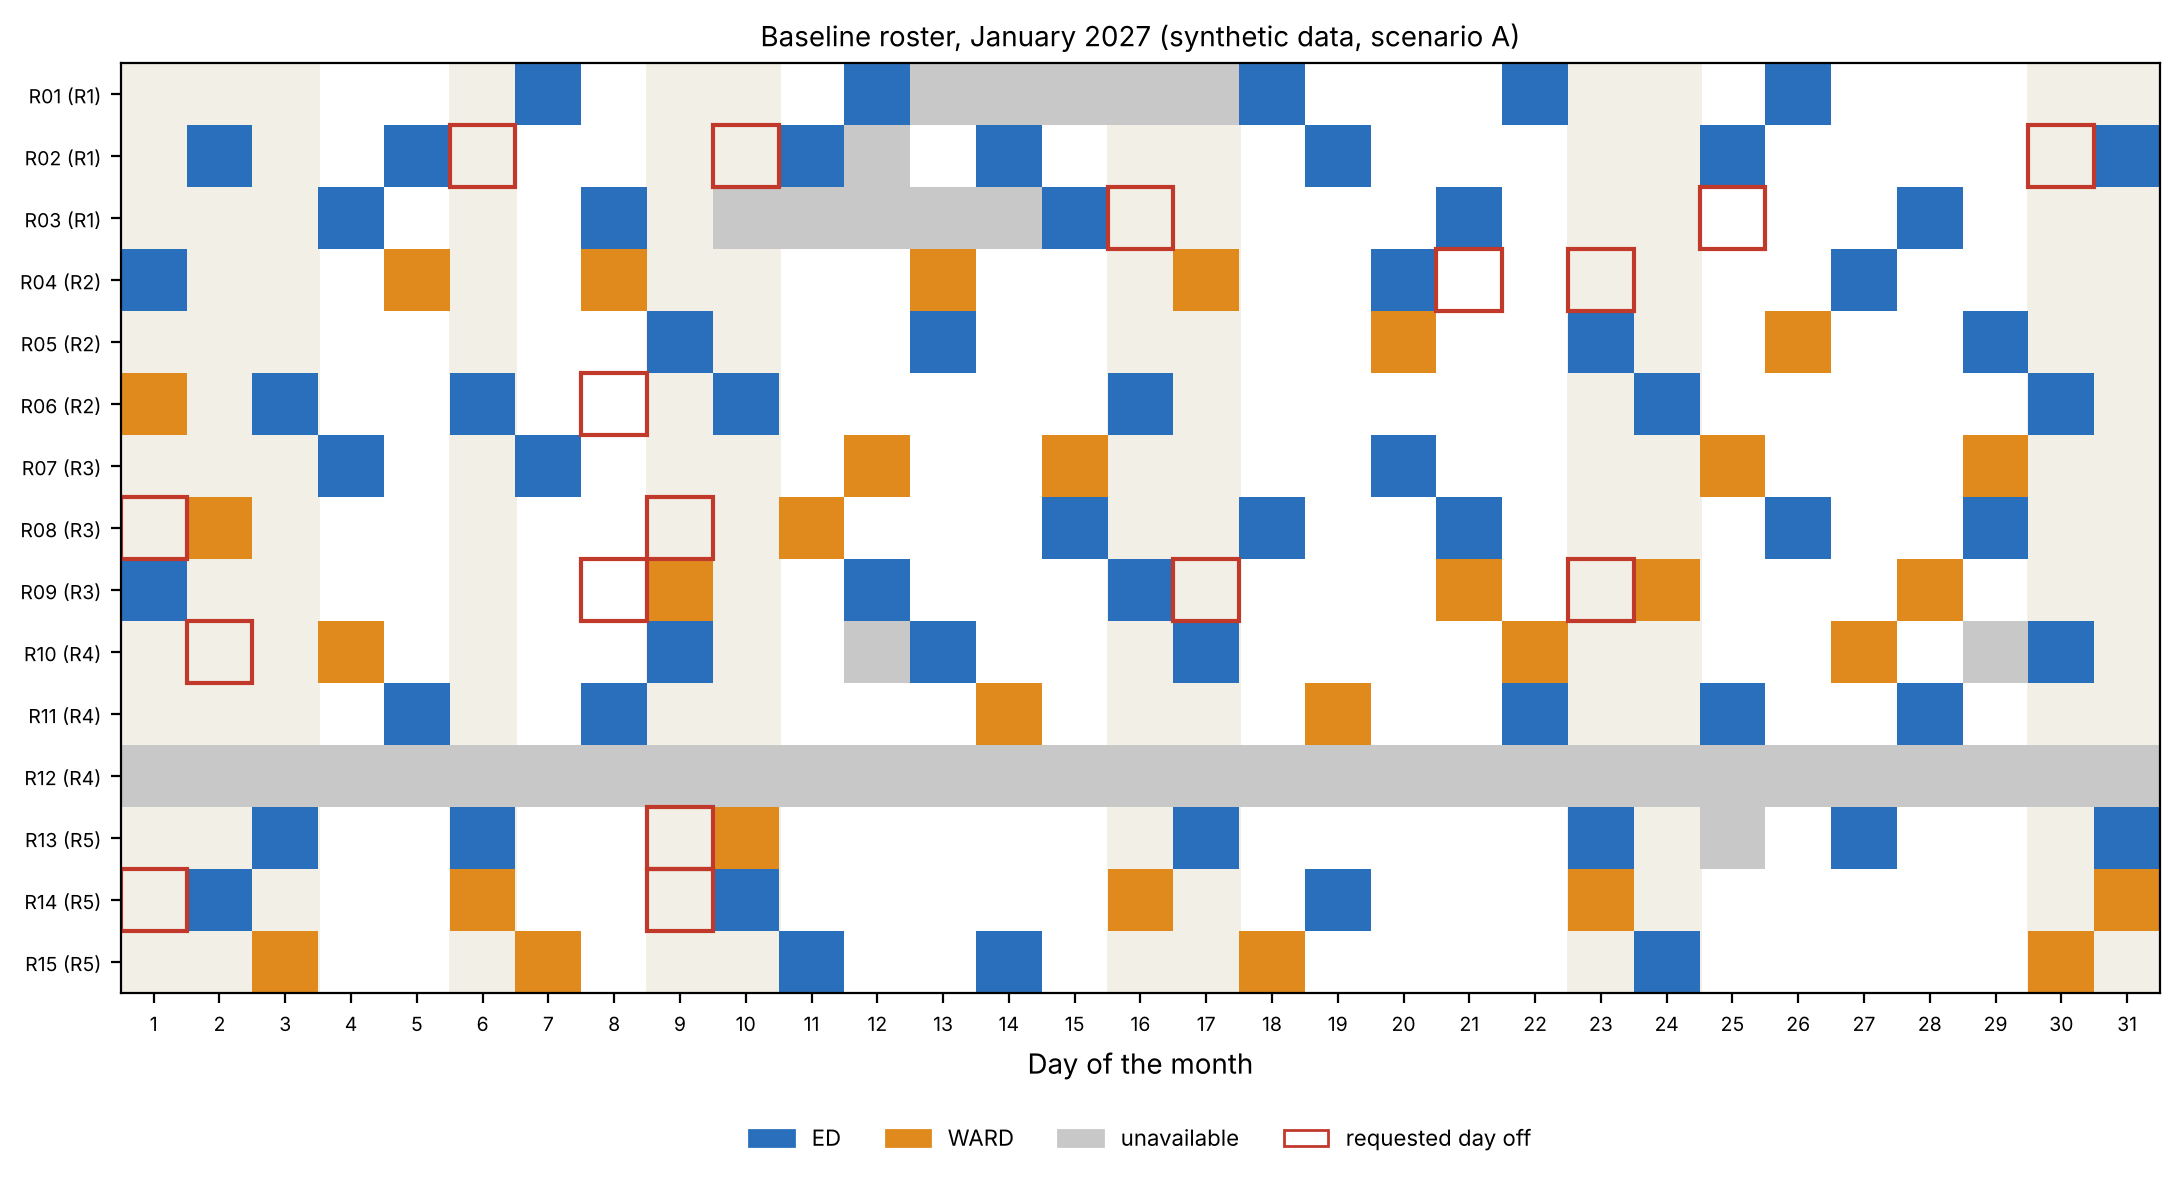
\includegraphics[width=0.92\linewidth]{roster_jan2027_base.png}
\vspace{-6pt}
\caption{\small Cuadrante óptimo de enero de 2027 (datos sintéticos, escenario A). Azul: urgencias; naranja: planta; gris: no disponible; recuadro rojo: día pedido libre; columnas sombreadas: fines de semana y festivos.}
\end{figure}

\textbf{Mes base.} En enero de 2027 el modelo cubre las 93 plazas sin déficit de mayores ni de personal de planta (nunca bajan de 9 residentes), respeta las 17 peticiones de días libres y deja un solo patrón «día sí, día no». Cada residente hace entre 5 y 7 guardias. La diferencia de carga normalizada de festivos baja de 21,7 a 14,8: el modelo asigna los festivos del mes a quienes llevaban menos (Figura~2).

\begin{figure}[h]
\centering
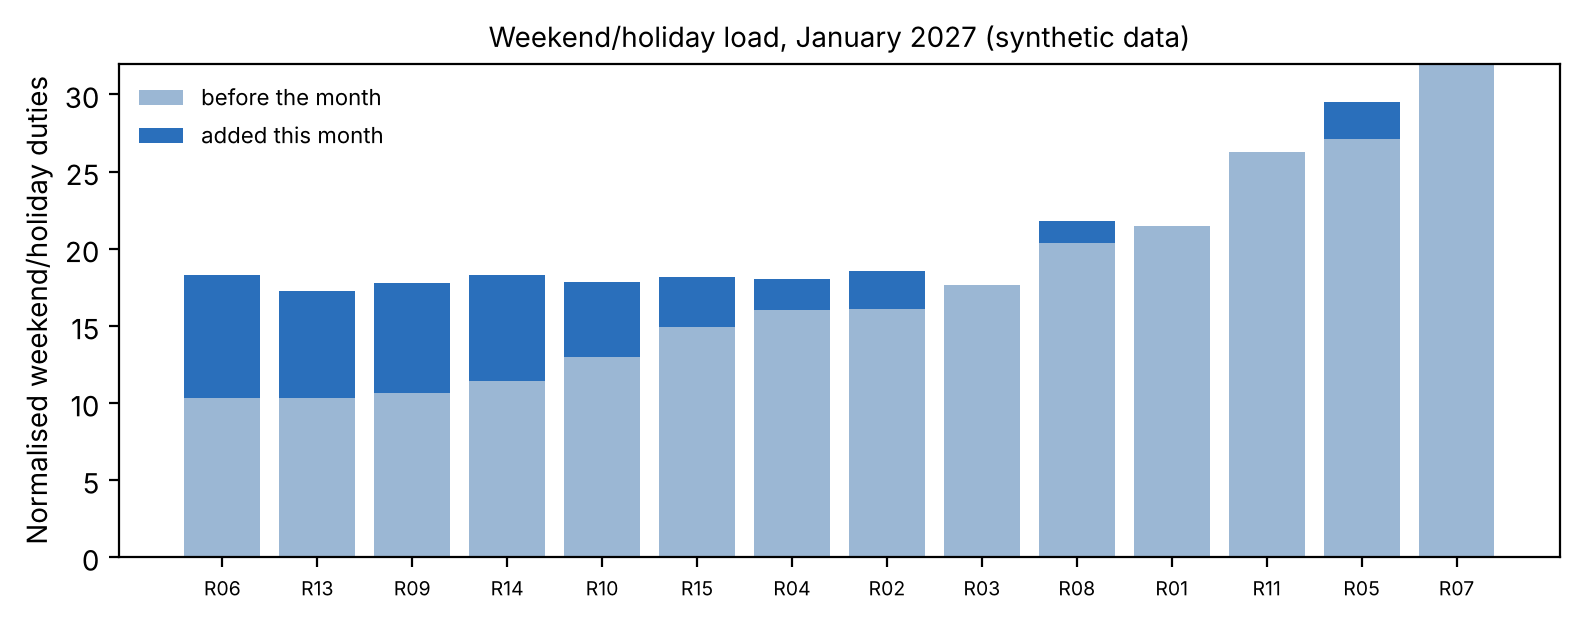
\includegraphics[width=0.62\linewidth]{fairness_jan2027_base.png}
\vspace{-6pt}
\caption{\small Carga normalizada de guardias en fin de semana o festivo antes del mes y añadida en enero.}
\end{figure}

\textbf{Primeras pruebas de estrés.}

\begin{center}\small
\begin{tabular}{@{}lccccccc@{}}
\toprule
 & Ene. base & Dic. Navidad & $-1$ res. & $-2$ res. & $-3$ res. & $-4$ res. & Esc. B (aprox.)\\
\midrule
Plazas de guardia sin cubrir & 0 & 5 & 2 & 9 & 20 & 32 & 37\\
Residentes que faltan en planta & 0 & 1 & 0 & 0 & 5 & 12 & 0\\
Peticiones incumplidas & 0/17 & 0/12 & 0/17 & 0/15 & 0/15 & 0/13 & 0/17\\
Rango de carga de festivos & 14,8 & 23,1 & 14,8 & 14,8 & 14,8 & 14,8 & 17,1\\
Guardias por residente & 5--7 & 3--7 & 7--7 & 7--7 & 4--7 & 3--7 & 4--4\\
\bottomrule
\end{tabular}
\end{center}

\begin{itemize}
  \item \textbf{El servicio está al límite.} Con un residente menos ya quedan 2 plazas sin cubrir y todos hacen el máximo de 7 guardias; con tres menos empieza a faltar personal de planta, porque cada guardia genera un saliente al día siguiente.
  \item \textbf{Diciembre} deja 5 plazas sin cubrir aunque la capacidad nominal sea la misma que en enero: las vacaciones concentradas y la regla de descanso reducen la capacidad real.
  \item \textbf{Escenario B.} Con un máximo de 4 guardias por residente, la plantilla actual solo cubre 56 de 93 plazas. Para cubrir este mes harían falta al menos 24 residentes disponibles ($93/4$), frente a los 14 actuales, sin contar que las guardias de 24~h de fin de semana tendrán que partirse en módulos más cortos. Es la pregunta central para el análisis final.
\end{itemize}

\section{Problemas encontrados y próximos pasos}

\begin{itemize}
  \item \textbf{Datos reales.} Seguimos sin autorización del hospital. Los supuestos (definición de mayor, guardia de tarde tras la jornada de mañana en el escenario~A, demanda, plantilla) deben validarse con el servicio.
  \item \textbf{Escenario B.} Para modelarlo bien necesitamos saber cómo reorganizará el servicio las guardias (tipos, duraciones $T_g$, horarios). Por ahora solo lo aproximamos con el máximo de 4 guardias.
  \item \textbf{Equidad con memoria.} El rango $e^{\max}-e^{\min}$ queda fijado por residentes con un histórico muy alto o muy bajo que un solo mes no puede compensar (14,8 en varios escenarios distintos). A partir de ese punto el objetivo no distingue entre los residentes intermedios. Compararemos métricas alternativas, como la desviación absoluta media respecto a la carga justa.
  \item \textbf{Pesos dentro de $f_1$.} Hoy una plaza sin cubrir y un residente menos en planta pesan igual. Hay que decidir con el servicio si una debe tener prioridad.
  \item \textbf{Licencia.} La licencia de Gurobi incluida con \texttt{pip} limita el modelo a 2\,000 variables y restricciones; las instancias actuales caben, pero para plantillas mayores necesitamos la licencia académica.
\end{itemize}

\textbf{Próximos pasos.} Análisis de sensibilidad completo (tamaño y composición de la plantilla, meses difíciles, métricas de equidad, prioridades de las peticiones y compromiso entre objetivos), escenario~B con guardias rediseñadas, y, si da tiempo, reprogramación ante ausencias imprevistas con el mínimo número de cambios.

\end{document}
